\subsection{Intérêt pour la compréhension des glaciations du quaternaire}

\paragraph{} Comme nous l'avons déjà souligné plus haut, un tel mécanisme d'amplification de petits forçage présente un certain attrait pour la théorie de Milankovitch. En effet, le problème des glaciations de la fin du quaternaire, espacées de 100\,kA, est que le principal cycle orbital candidat est celui de l'excentricité dont les composantes à 100\,kA ne font varier que peu le flux solaire (environ 0.1\% \cite{scholarpedia}). Le phénomène de résonance stochastique pourrait donc expliquer comment ce signal serait capable d'influencer le climat Terrestre. 

\paragraph{} Dans leurs articles du début des années 1980, Nicolis et Benzi étudient la variabilité du climat à travers ce qui appellent un potentiel climatique \cite{nicolis1982} \cite{benzi1983}. Cette grandeur joue le rôle du potentiel que ressent la particule dans nos dérivations ci-dessus. Le système étudié est dans ce cas-ci le climat Terrestre et son espace de configurations n'a qu'une seule variable, la température moyenne de la Terre\footnote{On parle de modèle zéro-dimensionnel lorsqu'aucune variable spatiale décrit le système.}. La dérivation d'un tel potentiel se fait à partir d'un bilan énergétique de la Terre (modèles dits de Budyko-Sellers). Les apports d'énergie sont le flux solaire et les pertes sont le rayonnement infrarouge ainsi que la réflexion des rayons solaires par la glace. L'équation bilan obtenue est du type

\begin{equation}\label{bilan_thermique}
	c\dv{T}{t} = R_{in}(T) - R_{out}(T) = Q_0(1-\alpha(T)) + \varepsilon \sigma T^4,
\end{equation}
où $c$ est la capacité calorifique de la Terre, $Q_0$ est le flux solaire moyen, $\alpha(T)$ l'albédo de la Terre en fonction de la température, $\varepsilon$ l'émissivité de la Terre et $\sigma$ la constante de Stefan.
         
\paragraph{} Dans son article, Nicolis utilise un modèle linéaire par morceaux pour la fonction albédo $\alpha(T)$ -- voir figure \ref{fig:bilan_thermique_albedo_lineaire}. La conclusion
\footnote{Sur une note personnelle: Comme expliqué dans l'article (\cite{nicolis1982}), le modèle utilisée pour la fonction albédo mène à des climats stables pour une Terre entièrement couverte de glace ainsi que le climat actuel. Il semble donc que ce modèle doit être encore raffiné pour expliquer les glaciations récentes, qui n'étaient que partielles.}
de son analyse est qu'on arrive à reproduire une résonance pour le cycle de 100\,kA. Du côté du groupe de Benzi, la fonction albédo est approximée par une forme présentant le double puits par construction et les paramètres sont ensuite ajustés pour que le modèle soit cohérent avec des résultats connus. Ce dernier groupe arrive aussi à la conclusion qu'une amplification par résonance stochastique est possible pour des valeurs de paramètres semblable à ceux du climat Terrestre. 

\paragraph{} Pour finir, malgré l'attrait que peut présenter le phénomène de résonance stochastique, il ne semble pas que de travaux plus récents ait permit de réserver un rôle essentiel au mécanisme pour faire le lien entre les cycles de Milankovitch et les glaciations quaternaires. Toutefois, une explication solide à ce lien est encore recherchée à ce jour. 

\begin{figure}
	\centering
	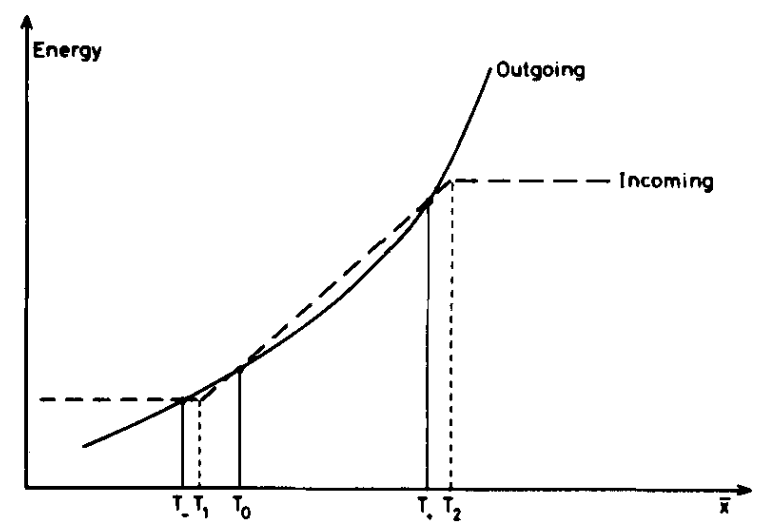
\includegraphics[width=0.8\linewidth]{figures/bilan_thermique_albedo_lineaire}
	\caption{Bilan énergétique suivant le modèle d'albédo linéaire par morceaux employé par Nicolis \cite{nicolis1982}. Image tirée de l'article.}
	\label{fig:bilan_thermique_albedo_lineaire}
\end{figure}

